%\使用前に、同ファイル内に「jrsj_UTF-8.cls」「rsj2021j_UTF-8.sty」を作成してからこのテンプレ―トを利用する
% \documentclass{jarticle}
\documentclass[a4paper]{jarticle}  % 210728: [a4paper]を追加
% \usepackage{rsj2021j}
\usepackage{rsj2021j_UTF-8}  % 210728: UTF-8で保存したものを使用
\usepackage[dvips]{graphicx}
\usepackage{url}

% \usepackage[utf8]{inputenc}  % 210728: 現時点では不要
\newpage  % 210728: 追加

\begin{document}
\title{第39回日本ロボット学会学術講演会 原稿の書き方}
\author{○信州太郎(日本ロボット学会)\ \ 東北花子((株)RSJ)}

\setlength{\baselineskip}{4.4mm} % 行間の設定
\maketitle
% \thispagestyle{empty}  % 210728: コメント化
% \pagestyle{empty}  % 210728: コメント化

\section{講演論文原稿作成方法について}
\begin{enumerate}
  \item {\bf 講演会ウェブサイトについて}
        講演論文原稿(PDF形式のみ)の投稿はインターネット経由で行います.
        詳細については,第39回日本ロボット学会学術講演会のウェブサイト\cite{website}をご参照ください.

  \item {\bf Microsoft Word 2000以降の場合}
        ウェブサイト\cite{website}から\verb|sample2021j.doc| をダウンロードして講演論文原稿を作成してください.
        MS WordやOSのバージョンによってはレイアウトが崩れる場合があります.

        そういった場合は,適宜 \verb|sample2021j.pdf| の書式に合うように原稿を作成してください.

  \item {\bf \TeX の場合}
        platex2eをお使いの方は,\verb|sample2021j.zip| をダウンロードし,
        中の \verb|sample2021j.tex| と \verb|rsj2021j.sty| をお使いください.
        なお,\TeX では,\verb|sample2021j.pdf|の書式とは異なる場合がございます.ご了承ください.

  \item {\bf その他の場合}
        \verb|sample2021j.pdf|の書式に合うように原稿を作成してください.
\end{enumerate}

作成したファイル(dviファイル,Wordファイル等)からPDFファイルを作成してください.
このときの画質,セキュリティ,余白等について注意してください.詳細は,ウェブサイト\cite{website}をご参照ください.
また,作成された PDFファイルを Adobe Acrobat Reader(旧 Adobe Reader)で開いてご確認ください.確認事項については,ウェブサイト\cite{website}をご参照ください.

\section{講演論文原稿書式について}
\subsection{原稿枚数について}
講演論文原稿は1ページ以上4ページ以内です.
ファイルの容量は3Mバイト(動画を含む場合は,動画を含めて4Mバイト)までです.
規定ページを越えるものは掲載いたしません.また,容量制限をこえるものは投稿できません.

\subsection{和文原稿の場合}
\subsubsection{原稿の体裁}
A4版白紙に縦250mm,横170mmの枠内に収まるようにお願いします.
主要活字は10ポイント以上をご使用ください.
提出された講演論文原稿は,そのまま予稿集に掲載いたします.
原稿の書き方が不適当にならないようにご留意ください.
詳細については,ウェブサイト\cite{website}をご参照ください.
\subsubsection{図と表について}
図・表は,印刷しても問題ない程度の解像度を持ち,
かつアップロードの際のファイルサイズ上限を越えない大きさとなるようにご留意ください.
\subsubsection{参考文献}
文献の引用は本文中に\cite{yamada2000}のように書き,
参考文献を本文の最後にまとめて書いてください.
参考文献の書式は,日本ロボット学会誌に準拠させてください.

\subsection{注意点}
2011年より,和文原稿には,英文題目,英文著者名を掲載しないことになりました.
図中のキャプションや図名も和文と致します.
また,和文,英文原稿ともアブストラクトおよびキーワードの掲載を求めないことにいたしました.

\subsection{英文原稿の場合}
英文原稿の執筆要綱は和文原稿のそれに準じます.
英文による題目,著者名をご記入下さい.
和文による題目,著者名等は不要です.

%図の入れ方
\begin{figure}[tb]
  \centering
  %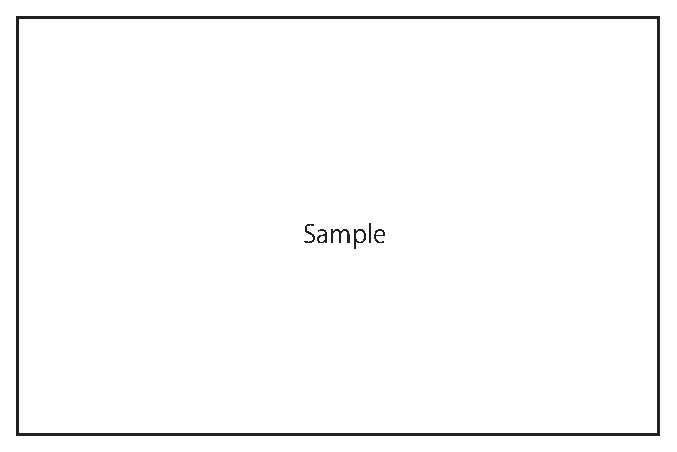
\includegraphics[width=45mm]{210520_samplefig2.eps}
  \caption{サンプル画像}
  \label{fig:sample}
\end{figure}

\section{講演申し込みおよび電子入稿}
2019年より講演申し込みと電子入稿の締め切りが異なり,2段階での手続きと
なりました.講演申込締切までに,講演題目・著者名・講演概要などを登録し,
講演の申し込みをしてください.その後,論文投稿〆切日までに,講演論文原稿ファイル(PDF形式)をアップロードして頂きます.詳細については,ウェブサイトをご参照ください.

\section{レター同時投稿について}

日本ロボット学会誌会誌編集委員会では,令和元年末に論文投稿規定の見直しを行いました.
この見直しに伴い,本講演会からレター同時投稿を受け付けることとなりました.
具体的には,日本ロボット学会学術講演会に投稿した講演論文を,「そのまま」の内容でレター(速報性を有する研究報告.最大4ページ)に投稿することが可能となりましたので,これを同時に受け付けます.
(ただし,フォーマットは異なります.)レター原稿の作成と投稿に関する詳細については,RSJのウェブサイトにあるPDF\cite{rsj_rules}
をご覧頂ければと思いますが,講演会の論文投稿と同時に,ロボット学会HPに掲載の論文投稿システムより,同内容をレターフォーマットで投稿して頂ければ,査読プロセス(速報性を重視するため初回査読期間は15日以内)を経てAcceptされた論文が,講演会後に順次オンラインに掲載されます.
学術講演会等の講演論文を論文誌に投稿する際には「新たな内容の追加や内容の充実が必要である」としていますが,日本ロボット学会が主催する学術講演会については,この規定の対象外としたため,レター同時投稿が可能となりました.この機会を使って,是非,レター投稿をご検討下さい. なお,レターは最大4ページですが,4ページ未満の原稿も受け付けます.

レター同時投稿の原稿作成ならびに投稿については,ウェブサイト\cite{website}をご参照ください.

%% 謝辞(必要な場合のみ)
%\begin{acknowledgements}
%    Thanks.
%\end{acknowledgements}

\small
\begin{thebibliography}{9}
  %%%%%%%%%%%%%%%%%%%%%%%%%%%%%%%%%%%%%%%%%%%%%%%%%%%%%%%%%%%%%%%%%%%%%%%%%%%%%%%

  \bibitem{yamada2000}
  山田太郎,鈴木一郎:
  ``第100回日本ロボット学会講演会用原稿の書き方'',
  日本ロボット学会誌,vol. 99,no. 4,pp. 8--12,2082.
  \bibitem{website}
  ``第39回日本ロボット学会学術講演会のウェブサイト'',
  \url{https: //ac.rsj-web.org/2021/}
  \bibitem{rsj_rules}
  ``日本ロボット学会誌・寄稿および査読に関する規則集'',
  \url{https: //www.rsj.or.jp/content/files/data_rules/F-02.pdf}

  %%%%%%%%%%%%%%%%%%%%%%%%%%%%%%%%%%%%%%%%%%%%%%%%%%%%%%%%%%%%%%%%%%%%%%%%%%%%%%%
\end{thebibliography}
\normalsize


\end{document}
